\documentclass[twocolumn]{article}
\usepackage[utf8]{inputenc}
\usepackage{math-symb}

\usepackage{tikz}

\usepackage[inline, shortlabels]{enumitem}
\setlist[itemize,1]{label=\rule[0.5ex]{0.5ex}{0.5ex}}
\setlist[itemize,2]{label=--}
\setlist[enumerate, 1]{label={\textbf{\arabic*.}}}
\setlist[enumerate, 2]{label={\roman*.}}

\usepackage{fancyhdr}
\pagestyle{fancy}
\fancyhf{}
\setlength{\headheight}{14pt}
\rhead{\textsc{Chapter II}}
\lhead{\textsc{A First Course In Probability}}
\rfoot{\textsc{9$^{\textsc{th}}$ edition}}
\cfoot{\thepage}

\DeclareMathSymbol{*}{\mathbin}{symbols}{"01}
\newcommand{\enquote}[1]{``#1''}

\begin{document}

\section*{Practical Problems}
\begin{enumerate}
    \item  A cafeteria offers a three-course meal consisting of an entree, a starch, and a dessert. The possible choices aregiven in the following table

\[
{
\begin{tabular}{ll}
    \hline
    \multicolumn{1}{c}{Course} & \multicolumn{1}{c}{Choices} \\
    \hline
    Entree & Chicken Roast, Roast Beef\\
    Starch & Pasta, rice, potatoes\\
    Dessert & Ice cream, Jello, apple pie, a peach\\
    \hline
\end{tabular}
}
\]
A person is to choose one course from each category.
\begin{enumerate}
    \item How many outcomes are in the sample space?
    \[ 2 * 3 * 4 \]
    \item Let $A$ be the event that ice cream is chosen. How many outcomes are in $A$?
    \[ 2 * 3 \]
    \item Let $B$ be the event that chicken is chosen. How many outcomes are in $B$?
    \[ 3 * 4 \]
    \item List all the outcomes in the event $AB$.
    \begin{align*}
        AB = \{ &\text{(chicken, pasta, ice-cream)},\\
        &\text{(chicken, rice, ice-cream)},\\
        &\text{(chicken, potatoes, ice-cream)} \}
    \end{align*}
    \item Let $C$ be the event that rice is chosen. How many outcomes are in $C$?
    \[ 2 * 4 \]
    \item List all the outcomes in the event $ABC$.
    \[ ABC = \{ \text{(chicken, rice, ice-cream)} \} \]
\end{enumerate}

    \item If 4 Americans, 3 French people, and 3 British people are to be seated in a row, how many seating arrangements are possible when people of the same nationality must sit next to each other?
\[ 4! * 3! * 3! * 3! \]
    \item $F = FE \cup FE^\complement $ and $E \cup F = E \cup E^\complement F$.

\begin{proof}[Demostración] de la relación anterior.

    \begin{align*}
        F &= FS\\
        &= F (E\cup E^\complement )\\
        &= FE \cup F E^\complement 
        \shortintertext{y}
        E \cup F &= (E \cup F)(E\cup E^\complement )\\
        &= ((E\cup F)E) \cup ((E\cup F)E^\complement )\\
        &= E \cup ((E^\complement  E)\cup(E^\complement  F))\\
        &= E \cup (\varnothing\cup(E^\complement  F))\\
        &= E \cup E^\complement  F \qedhere
    \end{align*}
\end{proof}
    \item $A$, $B$, and $C$ take turns flipping a coin. The first one to get a head wins. The sample space of this experiment can be defined by
\[ S = \begin{cases}
    1, 01, 001, 0001, \dots,\\
    0000\cdots
\end{cases} \]
\begin{enumerate}
    \item Interpret the sample space.
    
    Es el conjunto de secuencias formadas por 0 y 1, donde el $i$-ésimo componente representa el resultado de la tirada $i$-ésima, con 0 representando que el resultado es ceca y 1 representando que el resultado es cara. 
    
    \item Define the following events in terms of $S$, assuming that $A$ flips first, then $B$, then $C$, $\dots$
    \begin{enumerate}[label={\alph*.}]
        \item $A \text{ wins} = A.$
        \[ A = \set{ 1, 0001, 0000001, \dots } \]
        \item $B \text{ wins} = B.$
        \[ B = \set{ 01, 00001, 00000001, \dots } \]
        \item $(A \cup B)^\complement $
        \[ (A \cup B)^\complement  = \begin{cases}
            &001, 000001, \dots\\
            &0000\cdots
        \end{cases} \]
    \end{enumerate}
\end{enumerate}
    \item An ordinary deck of 52 cards is shuffled. What is the probability that the top four cards have
\begin{enumerate}
    \item different denominations?
    \[ \frac{\binom{13}{4}\binom{4}{1}^4}{\binom{52}{4}} \]
    \item different suits?
    \[ \frac{\binom{13}{1}^4}{\binom{52}{4}} \]
\end{enumerate}

    \item How many vectors $x_1, \dots, x_k$ are there for which each $x_i$ is a positive integer such that $1 \le x_i \le n$ and $x_1 < x_2 < \dots < x_k$?

Seleccionar los $k+i$ primeros números, y entre ellos asignar a $i$ el estatus de \enquote{ignorado}.
\[ \sum_{i=0}^{n-k} \binom{k+i}{i} \]
    \item Use Venn diagrams
\begin{enumerate}
    \item to simplify $(E \cup F)(E \cup F^c)$
    \[
    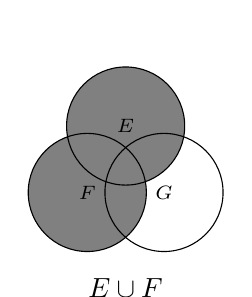
\begin{tikzpicture}[scale=0.75]
    \fill[fill=black!50] ( 90:.75) circle (1) (210:.75) circle (1);
    \foreach \a/\l in {90/E,210/F,330/G} {
        \path[draw] ++(\a:.75) circle (1) node {$\scriptstyle \l$};
    }
    \node at (0, -2) {$E \cup F$};
    \end{tikzpicture}
    \hspace{1em}
    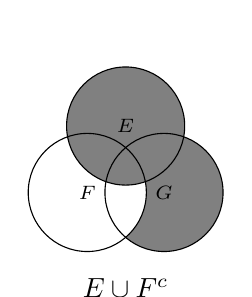
\begin{tikzpicture}[scale=0.75]
    \fill[fill=black!50] (90:.75) circle (1);
    \scope[even odd rule]
        \clip ( 90:.75) circle (1) (330:.75) circle (1);
        \clip (210:.75) circle (1) (330:.75) circle (1);
        \fill[fill=black!50] (330:.75) circle (1);
    \endscope
    \foreach \a/\l in {90/E,210/F,330/G} {
        \path[draw] ++(\a:.75) circle (1) node {$\scriptstyle \l$};
    }
    \node at (0, -2) {$E \cup F^c$};
    \end{tikzpicture}
    \]
    su intersección
    \[
    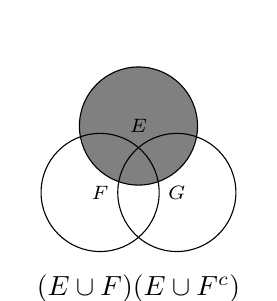
\begin{tikzpicture}[scale=0.75]
    \fill[fill=black!50] (90:.75) circle (1);
    \foreach \a/\l in {90/E,210/F,330/G} {
        \path[draw] ++(\a:.75) circle (1) node {$\scriptstyle \l$};
    }
    \node at (0, -2) {$(E \cup F) (E \cup F^c)$};
    \end{tikzpicture}
    \]
    \item to prove DeMorgan’s laws for events $E$ and $F$. (prove $(E \cup F)^c = E^cF^c$, and $(EF)^c = E^c \cup F^c$)

    \begin{proof}[Demostración] $(E \cup F)^c = E^cF^c$
        \[
        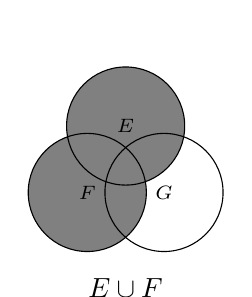
\begin{tikzpicture}[scale=0.75]
        \fill[fill=black!50] ( 90:.75) circle (1) (210:.75) circle (1);
        \foreach \a/\l in {90/E,210/F,330/G} {
            \path[draw] ++(\a:.75) circle (1) node {$\scriptstyle \l$};
        }
        \node at (0, -2) {$E \cup F$};
        \end{tikzpicture}
        \]
        su complemento
        \[
        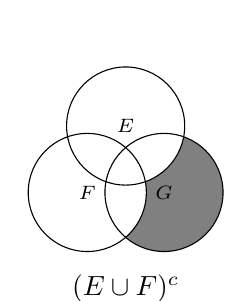
\begin{tikzpicture}[scale=0.75]
        \scope[even odd rule]
            \clip ( 90:.75) circle (1) (330:.75) circle (1);
            \clip (210:.75) circle (1) (330:.75) circle (1);
            \fill[fill=black!50] (330:.75) circle (1);
        \endscope
        \foreach \a/\l in {90/E,210/F,330/G} {
            \path[draw] ++(\a:.75) circle (1) node {$\scriptstyle \l$};
        }
        \node at (0, -2) {$(E \cup F)^c$};
        \end{tikzpicture}
        \]
        \[
        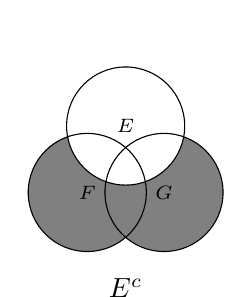
\begin{tikzpicture}[scale=0.75]
        \scope[even odd rule]
            \clip (210:.75) circle (1) (330:.75) circle (1);
            \clip ( 90:.75) circle (1) (210:.75) circle (1);
            \fill[fill=black!50] (210:.75) circle (1);
        \endscope
        \scope[even odd rule]
            \clip ( 90:.75) circle (1) (330:.75) circle (1);
            \fill[fill=black!50] (330:.75) circle (1);
        \endscope
        \foreach \a/\l in {90/E,210/F,330/G} {
            \path[draw] ++(\a:.75) circle (1) node {$\scriptstyle \l$};
        }
        \node at (0, -2) {$E^c$};
        \end{tikzpicture}
        \hspace{1em}
        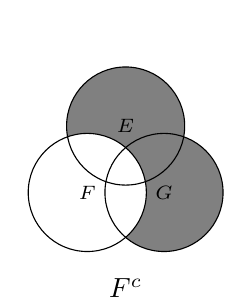
\begin{tikzpicture}[scale=0.75]
        \scope[even odd rule]
            \clip ( 90:.75) circle (1) (210:.75) circle (1);
            \clip (330:.75) circle (1) ( 90:.75) circle (1);
            \fill[fill=black!50] ( 90:.75) circle (1);
        \endscope
        \scope[even odd rule]
            \clip (210:.75) circle (1) (330:.75) circle (1);
            \fill[fill=black!50] (330:.75) circle (1);
        \endscope
        \foreach \a/\l in {90/E,210/F,330/G} {
            \path[draw] ++(\a:.75) circle (1) node {$\scriptstyle \l$};
        }
        \node at (0, -2) {$F^c$};
        \end{tikzpicture}
        \]
        su intersección
        \[
        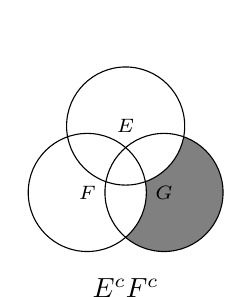
\begin{tikzpicture}[scale=0.75]
        \scope[even odd rule]
            \clip ( 90:.75) circle (1) (330:.75) circle (1);
            \clip (210:.75) circle (1) (330:.75) circle (1);
            \fill[fill=black!50] (330:.75) circle (1);
        \endscope
        \foreach \a/\l in {90/E,210/F,330/G} {
            \path[draw] ++(\a:.75) circle (1) node {$\scriptstyle \l$};
        }
        \node at (0, -2) {$E^c F^c$};
        \end{tikzpicture}
        \qedhere \]
    \end{proof}
    
    
    \begin{proof}[Demostración] $(EF)^c = E^c \cup F^c$
        \[
        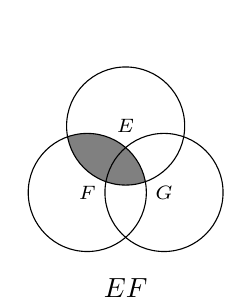
\begin{tikzpicture}[scale=0.75]
        \scope
            \clip (210:.75) circle (1);
            \fill[fill=black!50] ( 90:.75) circle (1);
        \endscope
        \foreach \a/\l in {90/E,210/F,330/G} {
            \path[draw] ++(\a:.75) circle (1) node {$\scriptstyle \l$};
        }
        \node at (0, -2) {$EF$};
        \end{tikzpicture}
        \]
        su complemento
        \[
        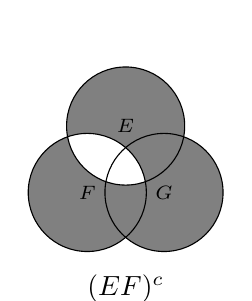
\begin{tikzpicture}[scale=0.75]
        \scope[even odd rule]
            \clip ( 90:.75) circle (1) (210:.75) circle (1);
            \fill[fill=black!50] (210:.75) circle (1);
        \endscope
        \scope[even odd rule]
            \clip ( 90:.75) circle (1) (210:.75) circle (1);
            \fill[fill=black!50] (90:.75) circle (1);
        \endscope
        \scope[even odd rule]
            \clip ( 90:.75) circle (1) (330:.75) circle (1);
            \clip (210:.75) circle (1) (330:.75) circle (1);
            \fill[fill=black!50] (330:.75) circle (1);
        \endscope
        \foreach \a/\l in {90/E,210/F,330/G} {
            \path[draw] ++(\a:.75) circle (1) node {$\scriptstyle \l$};
        }
        \node at (0, -2) {$(EF)^c$};
        \end{tikzpicture}
        \]
        \[
        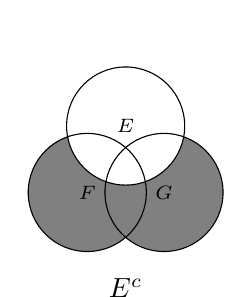
\begin{tikzpicture}[scale=0.75]
        \scope[even odd rule]
            \clip (210:.75) circle (1) (330:.75) circle (1);
            \clip ( 90:.75) circle (1) (210:.75) circle (1);
            \fill[fill=black!50] (210:.75) circle (1);
        \endscope
        \scope[even odd rule]
            \clip ( 90:.75) circle (1) (330:.75) circle (1);
            \fill[fill=black!50] (330:.75) circle (1);
        \endscope
        \foreach \a/\l in {90/E,210/F,330/G} {
            \path[draw] ++(\a:.75) circle (1) node {$\scriptstyle \l$};
        }
        \node at (0, -2) {$E^c$};
        \end{tikzpicture}
        \hspace{1em}
        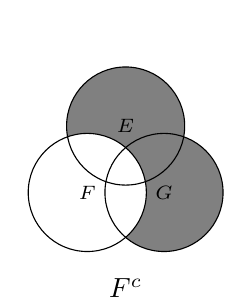
\begin{tikzpicture}[scale=0.75]
        \scope[even odd rule]
            \clip ( 90:.75) circle (1) (210:.75) circle (1);
            \clip (330:.75) circle (1) ( 90:.75) circle (1);
            \fill[fill=black!50] ( 90:.75) circle (1);
        \endscope
        \scope[even odd rule]
            \clip (210:.75) circle (1) (330:.75) circle (1);
            \fill[fill=black!50] (330:.75) circle (1);
        \endscope
        \foreach \a/\l in {90/E,210/F,330/G} {
            \path[draw] ++(\a:.75) circle (1) node {$\scriptstyle \l$};
        }
        \node at (0, -2) {$F^c$};
        \end{tikzpicture}
        \]
        su unión
        \[
        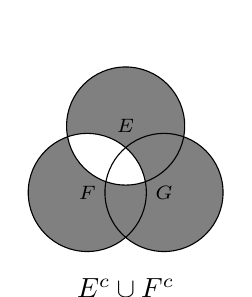
\begin{tikzpicture}[scale=0.75]
        \scope[even odd rule]
            \clip ( 90:.75) circle (1) (210:.75) circle (1);
            \fill[fill=black!50] (210:.75) circle (1);
        \endscope
        \scope[even odd rule]
            \clip ( 90:.75) circle (1) (210:.75) circle (1);
            \fill[fill=black!50] (90:.75) circle (1);
        \endscope
        \scope[even odd rule]
            \clip ( 90:.75) circle (1) (330:.75) circle (1);
            \clip (210:.75) circle (1) (330:.75) circle (1);
            \fill[fill=black!50] (330:.75) circle (1);
        \endscope
        \foreach \a/\l in {90/E,210/F,330/G} {
            \path[draw] ++(\a:.75) circle (1) node {$\scriptstyle \l$};
        }
        \node at (0, -2) {$E^c \cup F^c$};
        \end{tikzpicture} \qedhere
        \]
    \end{proof}
    
    
\end{enumerate}

    \item Suppose that $A$ and $B$ are mutually exclusive events for which $P(A) = .3$ and $P(B) = .5$. What is the probability that
\begin{enumerate}
    \item either $A$ or $B$ occurs?
    \begin{align*}
        P(A\cup B)
        &= P(A) + P(B)\\
        &= .3 + .5\\
        &= .8
    \end{align*}
    \item $A$ occurs but $B$ does not?
    \begin{align*}
        P(AB^\complement )
        &= P(A) - P(AB)\\
        &= .3 - .0\\
        &= .3
    \end{align*}
    \item both $A$ and $B$ occur?
    \begin{align*}
        P(AB) &= 0
    \end{align*}
\end{enumerate}
    \item A retail establishment accepts either the American Express or the VISA credit card. A total of 24 percent of its customers carry an American Express card, 61 percent carry a VISA card, and 11 percent carry both cards. What percentage of its customers carry a credit card that the establishment will accept?
\begin{align*}
    P(A\cup V) &= P(A) + P(V) - P(A \cap V)\\
    &= .24 + .61 - .11\\
    &= .74
\end{align*}
    \item In how many ways can 8 people be seated in a row if
\begin{enumerate}
    \item there are no restrictions on the seating arrangement?
    \[ 8! \]
    \item persons A and B must sit next to each other?
    \[ 2 * 7!\]
    \item there are 4 men and 4 women and no 2 men or 2 women can sit next to each other?

    Siguiendo la lógica de 7. iv.
    \[ 8 * 4 * 3 * 3 * 2 * 2 \]
    \item there are 5 men and they must sit next to one another?

    Hay $5!$ formas de sentar a los hombres entre sí, luego $4!$ formas de ordenar el grupo de hombres y las 3 mujeres.
    \[ 5! * 4! \]
    
    \item there are 4 married couples and each couple must sit together?

    Cada pareja tiene 2 formas de sentarse, luego hay $4!$ formas de ubicar a las parejas.
    \[ 2^4 * 4! \]
\end{enumerate}
    \item In how many ways can 3 novels, 2 mathematics books, and 1 chemistry book be arranged on a bookshelf if
\begin{enumerate}
    \item the books can be arranged in any order?
    \[ 6! \]
    \item the mathematics books must be together and the novels must be together?
    \[ 3! * 2! * 3! \]
    \item the novels must be together, but the other books can be arranged in any order?
    \[ 3! * 4! \]
\end{enumerate}
    \item A basketball team consists of 6 frontcourt and 4 backcourt players. If players are divided into roommates at random, what is the probability that there will be exactly two roommate pairs made up of a backcourt and a frontcourt player?
\[ \frac{\binom{6}{2} \binom{4}{2} * 2 * 3}{\frac{\binom{10}{2,2,2,2,2}}{5!}} \]
    \item Suppose that a person chooses a letter at random from R\,E\,S\,E\,R\,V\,E and then chooses one at random from \,V\,E\,R\,T\,I\,C\,A\,L. What is the probability that the same letter is chosen?
\[ 
\tfrac{2}{7} * \tfrac{1}{8} + \tfrac{3}{7} * \tfrac{1}{8} +
\tfrac{1}{7} * \tfrac{0}{8} + \tfrac{1}{7} * \tfrac{1}{8} = \tfrac{3}{28}  \]
    \item From a set of $n$ people, a committee of size $j$ is to be chosen, and from this committee, a subcommittee of size $i$, $i \le j$ is also to be chosen.
\begin{enumerate}
    \item Derive a combinatorial identity by computing, in two ways, the number of possible choices of the committee and subcommittee—first by supposing that the committee is chosen first and then the subcommittee is chosen, and second by supposing that the subcommittee is chosen first and then the remaining members of the committee are chosen.
    
    Supongamos que primero seleccionamos el comité, hay $\displaystyle \binom{n}{j}$ posibles comités, y de estas $j$ personas debemos seleccionar $i$ para que formen parte del subcomité
    \[ \binom{n}{j} * \binom{j}{i} \]

    Supongamos que primero seleccionamos el subcomité, hay $\displaystyle \binom{n}{i}$ posibles subcomités, luego de las restantes $n-i$ personas debemos seleccionar $j-i$
    \[ \binom{n}{i} * \binom{n-i}{j-i} \]

    Finalmente concluimos que
    \[ \binom{n}{j} * \binom{j}{i} = \binom{n}{i} * \binom{n-i}{j-i} \]

    \item Use part i. to prove the following combinatorial identity:
    \[ \sum_{j=i}^n \binom{n}{j} \binom{j}{i} = \binom{n}{i} * 2^{n-i} \quad i \le n \]
    \begin{align*}
        \shortintertext{por el inciso i.}
        \sum_{j=i}^n \binom{n}{j} \binom{j}{i} &= \sum_{j=i}^n \binom{n}{i} \binom{n-i}{j-i}\\
        &= \binom{n}{i} \sum_{j=i}^n \binom{n-i}{j-i}\\
        &= \binom{n}{i} \sum_{k=0}^{n-i} \binom{n-i}{k}
        \shortintertext{la suma equivale a todos los posibles subconjuntos de un conjunto con $n-i$ elementos.}
        &= \binom{n}{i} * 2^{n-i}
    \end{align*}
    
    \item  Use part i. and Theoretical Exercise 13 to show that
    \[ \sum_{j=i}^n \binom{n}{j} \binom{j}{i} (-1)^{(n-j)} = 0 \quad i < n\]
    \begin{align*}
        \shortintertext{por el inciso i.}
        &\phantom{{}={}} \sum_{j=i}^n \binom{n}{j} \binom{j}{i} (-1)^{(n-j)}\\
        &= \sum_{j=i}^n \binom{n}{i} \binom{n-i}{j-i} (-1)^{(n-j)}
        \shortintertext{la suma equivale a todos los posibles subconjuntos de un conjunto con $n-i$ elementos.}
        &= \binom{n}{i} * 2^{n-i}
    \end{align*}
\end{enumerate}
    \item A total of $n$ students are enrolled in a review course for the actuarial examination in probability. The posted results of the examination will list the names of those who passed, in decreasing order of their scores. For instance, the posted result will be \enquote{Brown, Cho} if Brown and Cho are the only ones to pass, with Brown receiving the higher score. Assuming that all scores are distinct (no ties), how many posted results are possible?
\[
\sum_{i=0}^n \binom{n}{i} * i!
\]
    \item Poker dice is played by simultaneously rolling 5 dice. Show that
\begin{enumerate}
    \item $P$\{no two alike\} = .0926;
    \[ \frac{6!}{6^5} \]
    \item $P$\{one pair\} = .4630;
    \[ \frac{\binom{6}{1} * 5 * 4 * 3 * \binom{5}{2}}{6^6} \]
    \item $P$\{two pair\} = .2315;
    \[ \frac{\binom{6}{2} * 4 * \frac{5!}{2!*2!}}{6^5} \]
    \item $P$\{three alike\} = .1543;
    \[ \frac{\binom{6}{1} * 5 * 4 * \binom{5}{3}}{6^5} \]
    \item $P$\{full house\} = .0386;
    \[ \frac{6 * 5 * \binom{5}{3}}{6^5} \]
    \item $P$\{four alike\} = .0193;
    \[ \frac{6 * 5 * 5}{6^5} \]
    \item $P$\{five alike\} = .0008.
    \[ \frac{6}{6^5} \]
\end{enumerate}
    \item Present a combinatorial explanation of why
\[ \binom{n}{r} = \binom{n}{r, n-r} \]

Al seleccionar $r$ objetos entre $n$ objetos queda únicamente determinado otro grupo de $n-r$ objetos, los que no fueron seleccionados.
    \item Two cards are randomly selected from an ordinary playing deck. What is the probability that they form a blackjack? That is, what is the probability that one of the cards is an ace and the other one is either a ten, a jack, a queen, or a king?
\[
\frac{4 * 4 * 4}{\binom{52}{2}}
\]
    \item If there are no restrictions on where the digits and letters are placed, how many 8-place license plates consisting of 5 letters and 3 digits are possible if no repetitions of letters or digits are allowed? What if the 3 digits must be consecutive?
\[ \binom{8}{3} * \frac{26!}{21!} * \frac{10!}{7!} \]
Si los 3 dígitos deben ser consecutivos entonces
\[ 6 * \frac{26!}{21!} * \frac{10!}{7!} \]
    \item In how many ways can $n$ identical balls be distributed into $r$ urns so that the $i$th urn contains at least $m_i$ balls for each $i = 1,\dots,r$? Assume that $n \ge \sum_{i=1}^r m_i$.

Primero colocamos las bolillas requeridas en las urnas, y nos restan $n - \sum_{i=1}^r m_i$ bolillas.

Luego debemos colocar las $n - \sum_{i=1}^r m_i$ bolillas restantes en las $r$ urnas
\[ \binom{ n + r - 1 - \sum_{i=1}^r m_i}{r-1} \]
    \item A small community organization consists of 20 families, of which 4 have one child, 8 have two children, 5 have three children, 2 have four children, and 1 has five children.

%4+2*8+3*5+4*2+5*1=20+23+5=48

\begin{enumerate}
    \item If one of these families is chosen at random, what is the probability it has $i$ children, $i = 1,2,3,4,5$?
    \[ 1.\ \frac{4}{20} \quad 2.\ \frac{8}{20} \quad 3.\ \frac{5}{20} \quad 4.\ \frac{2}{20} \quad 5.\ \frac{1}{20} \quad \]
    \item If one of the children is randomly chosen, what is the probability that child comes from a family having $i$ children, $i = 1,2,3,4,5$?
    \[ 1.\ \frac{4}{48} \quad 2.\ \frac{16}{48} \quad 3.\ \frac{15}{48} \quad 4.\ \frac{8}{48} \quad 5.\ \frac{5}{48} \quad \]
\end{enumerate}
    \item  Consider a function $f(x_1, \dots, x_n)$ of $n$ variables. How many different partial derivatives of order $r$ does $f$ posses?

Si asumimos que $f \in C^r$ entonces buscamos las soluciones a 
\[ a_1 + a_2 + \dots + a_n = r\quad x_i \ge 0, \quad i=1,\dots,n \]
Entonces
\[ \binom{r+n-1}{n-1} \]
    \item A pair of fair dice is rolled. What is the probability that the second die lands on a higher value than does the first?
\[
\frac{5+4+3+2+1+0}{6^2} = \frac{15}{6^2}
\]
    \item If two dice are rolled, what is the probability that the sum of the upturned faces equals $i$? Find it for $i = 2,3,\dots,11,12$.
\begin{alignat*}{6}
    &2.\ \frac{1}{6^2}\quad &&3.\ \frac{2}{6^2}\quad &&4.\ \frac{3}{6^2}\quad &&5.\ \frac{4}{6^2}\quad &&6.\ \frac{5}{6^2}\\
    &7.\ \frac{6}{6^2}\quad &&8.\ \frac{5}{6^2}\quad &&9.\ \frac{4}{6^2}\quad &&10.\ \frac{3}{6^2}\quad &&11.\ \frac{2}{6^2}\quad &&12.\ \frac{1}{6^2}
\end{alignat*}
    \item A pair of dice is rolled until a sum of either 5 or 7 appears. Find the probability that a 5 occurs first. 

\emph{Hint}: Let $E_n$ denote the event that a 5 occurs on the $n$th roll and no 5 or 7 occurs on the first $n - 1$ rolls. Compute $P(E_n)$ and argue that $\sum_{n=1}^\infty P(E_n)$ is the desired probability.

\begin{align*}
    &\phantom{{}={}} P(E_n)\\
    &= P(\{\text{no suma 5 o 7 en $n-1$ tiros}\}) * {}\\
    &\phantom{{}={}} P(\{\text{suma 5 o 7}\})\\
    &= \big(1 - P(\{\text{sumar 5 o 7}\})\big)^{n-1} *\\
    &\phantom{{}={}} P(\{\text{sumar 5 o 7}\})\\
    &= \bigg(\frac{26}{6^2}\bigg)^{n-1} * \frac{4}{6^2}
\shortintertext{entonces}
    &\phantom{{}={}} \sum_{i=1}^\infty P(E_n)\\
    &= \sum_{i=0}^\infty \bigg(\frac{26}{6^2}\bigg)^i * \frac{4}{6^2}\\
    &= \lim_{n\to\infty} \sum_{i=0}^n \bigg(\frac{26}{6^2}\bigg)^i * \frac{4}{6^2}\\
    &= \frac{4}{6^2} * \lim_{n\to\infty} \sum_{i=0}^n 
    \frac{26^i}{36^i}
    \shortintertext{por formula cerrada de serie geométrica}
    &= \frac{4}{6^2} * \lim_{n\to\infty} \frac{1 - (\frac{26}{36})^{n+1}}{1-\frac{26}{36}}\\
    &= \frac{4}{6^2} * \frac{1}{\frac{10}{36}}\\
    &= \frac{2}{5}
\end{align*}
    \item Expand $(x_1 + 2 x_2 + 3 x_3)^4$.

usando el teorema del multinomio $(x_1 + 2 x_2 + 3 x_3)^4$ equivale a
\[ \sum_{\substack{(n_1, n_2, n_3):\\n_1 + n_2 + n_3 = 4}} \binom{4}{n_1, n_2, n_3} * x_1^{n_1} * (2 x_2)^{n_2} * (3 x_3)^{n_3} \]
    \item If 12 people are to be divided into 3 committees of respective sizes 3, 4, and 5, how many divisions are possible?
\[ \binom{12}{3,4,5} \]
    \item  If 8 new teachers are to be divided among 4 schools, how many divisions are possible? What if each school must receive 2 teachers?
\[4^8\]
Si cada escuela debe recibir aunque sea 2 maestros
\[ \binom{8}{2,2,2,2} \]
    \item An urn contains $n$ white and $m$ black balls, where $n$ and $m$ are positive numbers.
\begin{enumerate}
    \item If two balls are randomly withdrawn, what is the probability that they are the same color?
    \[ \frac{\binom{n}{2} + \binom{m}{2}}{\binom{n+m}{2}} \]
    
    \item If a ball is randomly withdrawn and then replaced before the second one is drawn, what is the probability that the withdrawn balls are the same color?
    \[ \frac{n^2 + m^2}{(n+m)^2} \]
    
    \item Show that the probability in part ii. is always larger than the one in part i.

    i.\@ la probabilidad de seleccionar otra del mismo color es de $\frac{n-1}{n+m}$ o $\frac{m-1}{n+m}$ mientras que en ii.\@ la probabilidad es de $\frac{n}{n+m}$ o $\frac{m}{n+m}$.
\end{enumerate}
    \item The chess clubs of two schools consist of, respectively, 8 and 9 players. Four members from each club are randomly chosen to participate in a contest between the two schools. The chosen players from one team are then randomly paired with those from the other team, and each pairing plays a game of chess. Suppose that Rebecca and her sister Elise are on the chess clubs at different schools. What is the probability that
\begin{enumerate}
    \item Rebecca and Elise will be paired?
    \[ \frac{\binom{7}{3} * \binom{8}{3} * 3!}{\binom{8}{4} * \binom{9}{4} * 4!} \]
    \item Rebecca and Elise will be chosen to represent their schools but will not play each other?
    \[ \frac{\binom{7}{3} * \binom{8}{3} * (4! - 3!)}{\binom{8}{4} * \binom{9}{4} * 4!} \]
    \item either Rebecca or Elise will be chosen to represent her school?
    \[ \frac{\binom{7}{3} * \binom{8}{4} + \binom{7}{4} * \binom{8}{3}}{\binom{8}{4} * \binom{9}{4}}\]
\end{enumerate}
    \item If 8 identical blackboards are to be divided among 4 schools, how many divisions are possible? How many if each school must receive at least 1 blackboard?

Buscamos soluciones a
\[ x_1 + x_2 + x_3 + x_4 = 8,\ x_i \ge 0,\ 1 \le i \le 4 \]
entonces
\[ \binom{8+4-1}{4-1} \]
si cada escuela debe recibir aunque sea 1 pizarrón
\[ x_1 + x_2 + x_3 + x_4 = 8,\ x_i \ge 1,\ 1 \le i \le 4 \]
entonces
\[ \binom{8-1}{4-1} \]
    \item A group of individuals containing $b$ boys and $g$ girls is lined up in random order; that is, each of the $(b + g)!$ permutations is assumed to be equally likely. What is the probability that the person in the $i$th position, $1 \le i \le b + g$, is a girl?

Si fijamos el contenido de la posición $i$-ésima en chico entonces hay $\frac{(b+g-1)!}{(b-1)!*g!}$ permutaciones tal que la $i$-ésima posición es un chico. Si fijamos el contenido de la posición $i$-ésima en chica entonces hay $\frac{(b+g-1)!}{b!*(g-1)!}$ permutaciones tal que la $i$-ésima posición es una chica.

Por lo tanto la probabilidad de que la $i$-ésima posición sea una chica es de
\[ \frac{\frac{(b+g-1)!}{b!*(g-1)!}}{\frac{(b+g)!}{b! * g!}} 
= 
\frac{(b+g-1)! * b! * g!}{b!*(g-1)! * (b+g)!}
=
\frac{g}{b+g}
\]
    \item A forest contains 20 elk, of which 5 are captured, tagged, and then released. A certain time later, 4 of the 20 elk are captured. What is the probability that 2 of these 4 have been tagged? What assumptions are you making?

\[ \frac{\binom{5}{2} * \binom{15}{2}}{\binom{20}{4}} \]
Asumimos que los hechos son independientes.
    \item The second Earl of Yarborough is reported to have bet at odds of 1000 to 1 that a bridge hand of 13 cards would contain at least one card that is ten or higher. (By ten or higher we mean that a card is either a ten, a jack, a queen, a king, or an ace.) Nowadays, we call a hand that has no cards higher than 9 a Yarborough. What is the probability that a randomly selected bridge hand is a Yarborough?
\[ \frac{\binom{32}{13}}{\binom{52}{13}} \]
    \item Seven balls are randomly withdrawn from an urn that contains 12 red, 16 blue, and 18 green balls. Find the probability that
\begin{enumerate}
    \item 3 red, 2 blue, and 2 green balls are withdrawn;
    \[ \frac{\binom{12}{3} * \binom{16}{2} * \binom{18}{2}}{\binom{46}{7}} \]
    \item at least 2 red balls are withdrawn;
    \[ 1 - \frac{\binom{34}{7} + \binom{12}{1} * \binom{34}{6}}{\binom{46}{7}} \]
    \item all withdrawn balls are the same color;
    \[ \frac{\binom{12}{7}+\binom{16}{7}+\binom{18}{7}}{\binom{46}{7}} \]
    \item either exactly 3 red balls or exactly 3 blue balls are withdrawn.
    \begin{align*}
        &\frac{\binom{12}{3} * \Big(\binom{18}{2}*\binom{16}{2}+\binom{18}{3}*\binom{16}{1}+\binom{18}{4}\Big)}{\binom{46}{7}} + {}\\
        &\frac{\binom{16}{3} * \Big(\binom{18}{2}*\binom{12}{2}+\binom{18}{3}*\binom{12}{1}+\binom{18}{4}\Big)}{\binom{46}{7}}
    \end{align*}
\end{enumerate}
    \item Two cards are chosen at random from a deck of 52 playing cards. What is the probability that they
\begin{enumerate}
    \item are both aces?
    \[ \frac{\binom{4}{2}}{\binom{52}{2}} \]
    \item have the same value?
    \[ \frac{13 * \binom{4}{2}}{\binom{52}{2}} \]
\end{enumerate}
    \item An instructor gives her class a set of 10 problems with the information that the final exam will consist of a random selection of 5 of them. If a student has figured out how to do 7 of the problems, what is the probability that he or she will answer correctly
\begin{enumerate}
    \item all 5 problems?
    \[ \frac{\binom{7}{5}}{\binom{10}{5}} \]
    \item at least 4 of the problems?
    \[ 
    \frac{\binom{7}{4}*\binom{3}{1}}{\binom{10}{5}} 
    + 
    \frac{\binom{7}{5}}{\binom{10}{5}} \]
\end{enumerate}
    \item There are $n$ socks, 3 of which are red, in a drawer. What is the value of $n$ if, when 2 of the socks are chosen randomly, the probability that they are both red is $\frac{1}{2}$.
\begin{align*}
    \frac{1}{2} &= P(\{2 \text{ red}\})\\
    &= \frac{\binom{3}{2}}{\binom{n}{2}}\\
    &= \frac{3 * 2}{(n-1) * n}
    \shortintertext{entonces}
    (n-1) * n &= 12\\
    n &= 4
\end{align*}
    \item There are 5 hotels in a certain town. If 3 people check into hotels in a day, what is the probability that they each check into a different hotel? What assumptions are you making?
\[ \frac{5*4*3}{5^3} \]
Asumimos que los hechos son independientes.
    \item A town contains 4 people who repair televisions. If 4 sets break down, what is the probability that exactly $i$ of the repairers are called? Solve the problem for $i = 1,2,3,4$. What assumptions are you making?
\begin{alignat*}{2}
    &1.\ \frac{4}{4^4}\quad 
    &&2.\ \frac{\binom{4}{2} * \big(4 + \binom{4}{2} + 4 \big)}{4^4}\\
    &3.\ \frac{\binom{4}{3} * \binom{3}{1} * \frac{4!}{2!}}{4^4}\quad 
    &&4.\ \frac{4 * 3 * 2 * 1}{4^4}
\end{alignat*}
Asumimos que los hechos son independientes.
    \item If a die is rolled 4 times, what is the probability that 6 comes up at least once?
\[\frac{\binom{4}{1} * 5^3 + \binom{4}{2} * 5^2 + \binom{4}{3} * 5^1 + \binom{4}{4} * 5^0}{6^4} \]
    \item  Two dice are thrown $n$ times in succession. Compute the probability that double 6 appears at least once. How large need $n$ be to make this probability at least $\frac{1}{2}$?
\begin{align*}
    &1 - P(\{\text{no doble 6 en $n$ tiros}\})\\
    &1 - (\tfrac{35}{36})^n
\end{align*}
La probabilidad es mayor a $\tfrac{1}{2}$ cuando $(\tfrac{35}{36})^n$ sea menor a $\tfrac{1}{2}$. Esto sucede cuando $n \ge 25$.
    \item 
\begin{enumerate}
    \item If $N$ people, including $A$ and $B$, are randomly arranged in a line, what is the probability that $A$ and $B$ are next to each other?
    \[ \frac{2 * \binom{N-1}{1} * (N-2)!}{N!} = \frac{2}{N} \]
    \item What would the probability be if the people were randomly arranged in a circle?
    \[ \frac{N}{\binom{N}{2}} = \frac{2}{N-1} \]
\end{enumerate}
    \item Five people, designated as $A, B, C, D, E$, are arranged in linear order. Assuming that each possible order is equally likely, what is the probability that
\begin{enumerate}
    \item there is exactly one person between $A$ and $B$?
    \[ \frac{2 * \binom{3}{1} * 1! * 3!}{5!} \]
    \item there are exactly two people between $A$ and $B$?
    \[ \frac{2 * \binom{3}{2} * 2! * 2!}{5!} \]
    \item there are three people between $A$ and $B$?
    \[ \frac{2 * \binom{3}{3} * 3! * 1!}{5!} \]
\end{enumerate}
    \item A woman has $n$ keys, of which one will open her door.
\begin{enumerate}
    \item If she tries the keys at random, discarding those that do not work, what is the probability that she will open the door on her $k$th try?
    \[ \frac{1}{n} \]
    \item What if she does not discard previously tried keys?
    \[ \Big(\frac{n-1}{n}\Big)^{k-1} * \frac{1}{n} \]
\end{enumerate}
    \item How many people have to be in a room in order that the probability that at least two of them celebrate their birthday in the same month is at least $\tfrac{1}{2}$? Assume that all possible monthly outcomes are equally likely.

Para $1 \le n \le 12$
\begin{align*}
    1 - \frac{\frac{12!}{(12-n)!}}{12^n}
\end{align*}
Que es mayor a $\tfrac{1}{2}$ cuando $n \ge 5$.
    \item If there are 12 strangers in a room, what is the probability that no two of them celebrate their birthday in the same month?
\[ 
\frac{12!}{12^n}
\]
    \item Given 20 people, what is the probability that among the 12 months in the year, there are 4 months containing exactly 2 birthdays and 4 containing exactly 3 birthdays?
\[
\frac{\binom{20}{2,2,2,2,3,3,3,3,0,0,0,0} * \binom{12}{4,4,4}}{12^{20}}
\]
    \item A group of 6 men and 6 women is randomly divided into 2 groups of size 6 each. What is the probability that both groups will have the same number of men?
\[ \frac{\binom{6}{3} * \binom{6}{3}}{2^{12}} \]
    \item In a hand of bridge, find the probability that you have 5 spades and your partner has the remaining 8.
\[ \frac{\binom{13}{5,8} * \binom{39}{13} * \binom{13}{8,5}}{\binom{52}{26} * \binom{26}{13}} \]
    \item Suppose that $n$ balls are randomly distributed into $N$ compartments. Find the probability that $m$ balls will fall into the first compartment. Assume that all $N$ arrangements are equally likely.

\[ \frac{\binom{n}{m} * (N-1)^{n-m}}{N^n} \]
    \item A closet contains 10 pairs of shoes. If 8 shoes are randomly selected, what is the probability that there will be
\begin{enumerate}
    \item no complete pair?
    \[ \frac{\binom{10}{8} * 2^8}{\binom{20}{8}} \]
    \item exactly 1 complete pair?
    \[ \frac{\binom{10}{7} * \binom{7}{6} * 2^6}{\binom{20}{8}} \]
\end{enumerate}
    \item If 4 married couples are arranged in a row, find the probability that no husband sits next to his wife.

Sea $E_i$ el evento tal que exactamente $i$ parejas se sientan juntas, $i = 0,1,2,3,4$.
\begin{align*}
    &\phantom{{}={}} P(E_0)\\
    &= 1 - P(E_1 \cup E_2 \cup E_3 \cup E_4)\\
    &= 1 - \binom{4}{1} * \frac{2^1 * 7!}{8!} 
    +  \binom{4}{2} * \frac{2^2 * 6!}{8!}\\
    &\phantom{{}= 1} -
       \binom{4}{3} * \frac{2^3 * 5!}{8!} 
    +  \binom{4}{4} * \frac{2^4 * 4!}{8!}
\end{align*}
    \item Compute the probability that a bridge hand is void in at least one suit. Note that the answer is not
\[ \frac{\binom{4}{1} * \binom{39}{13}}{\binom{52}{13}} \]
Why not?

Los casos no son necesariamente disjuntos, hay manos que no tienen ninguna carta de dos o tres palos.

Sea $E_i$ el evento tal que la mano de bridge no tiene ninguna carta del palo $i$, $i = 1,2,3,4$.
\begin{align*}
    &\phantom{{}={}} P(E_1\cup E_2\cup E_3\cup E_4)\\
    &= \binom{4}{1} * \frac{\binom{39}{13}}{\binom{52}{13}}
    -  \binom{4}{2} * \frac{\binom{26}{13}}{\binom{52}{13}} + \binom{4}{3} * \frac{\binom{13}{13}}{\binom{52}{13}}
\end{align*}
    \item Compute the probability that a hand of 13 cards contains
\begin{enumerate}
    \item the ace and king of at least one suit.

   Sea $E_i$ el evento tal que la mano contiene el as y el rey del palo $i$, $i = 1,2,3,4$.
    \begin{align*}
        &\phantom{{}={}} P(E_1\cup E_2\cup E_3\cup E_4)\\
        &= \binom{4}{1} * \frac{\binom{50}{11}}{\binom{52}{13}}
        -  \binom{4}{2} * \frac{\binom{48}{ 9}}{\binom{52}{13}} + {}\\
        &\phantom{{}={}}
           \binom{4}{3} * \frac{\binom{46}{ 7}}{\binom{52}{13}} -
           \binom{4}{4} * \frac{\binom{44}{ 5}}{\binom{52}{13}}
    \end{align*}
    \item all 4 of at least 1 of the 13 denominations.

    Sea $E_i$ el evento tal que la mano contiene las cuatro cartas numeradas $i$, $i = 1,2,\dots,13$.
    \begin{align*}
        &\phantom{{}={}} P(\textstyle \bigcup_{i=1}^{13} E_i)\\
        &= \binom{13}{1} * \frac{\binom{48}{9}}{\binom{52}{13}}
        -  \binom{13}{2} * \frac{\binom{44}{ 5}}{\binom{52}{13}} + {}\\
        &\phantom{{}={}}
           \binom{13}{3} * \frac{\binom{40}{ 1}}{\binom{52}{13}}
    \end{align*}
\end{enumerate}
    \item Two players play the following game: Player $A$ chooses one of the three spinners pictured in Figure 6, and then player $B$ chooses one of the remaining two spinners. Both players then spin their spinner, and the one that lands on the higher number is declared the winner. Assuming that each spinner is equally likely to land in any of its 3 regions, would you rather be player $A$ or player $B$? Explain your answer!
\[
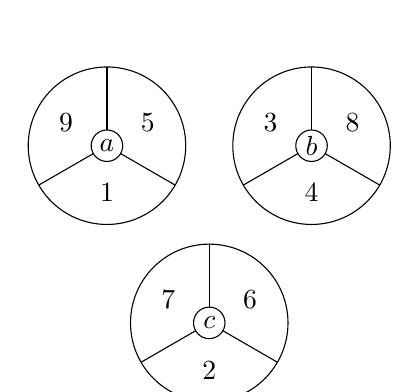
\begin{tikzpicture}
    \def \radius {1.5}
    \begin{scope}[shift={(150:\radius)}]
        \draw (0, 0) circle (1);
        \draw (0, 0) circle (0.2);
        \node at (0, 0) {$a$};
        \foreach \lineangle/\lblangle/\lbl in {90/150/9, 210/270/1, 330/30/5} {
            \draw (0, 0) +(\lineangle:.2) -- +(\lineangle:1);
            \path (0, 0) ++(\lblangle:.6) node {\lbl};
        }
    \end{scope}
    
    \begin{scope}[shift={(270:\radius)}]
        \draw (0, 0) circle (1);
        \draw (0, 0) circle (0.2);
        \node at (0, 0) {$c$};
        \foreach \lineangle/\lblangle/\lbl in {90/150/7, 210/270/2, 330/30/6} {
            \draw (0, 0) +(\lineangle:.2) -- +(\lineangle:1);
            \path (0, 0) ++(\lblangle:.6) node {\lbl};
        }
    \end{scope}

    \begin{scope}[shift={( 30:\radius)}]
        \draw (0, 0) circle (1);
        \draw (0, 0) circle (0.2);
        \node at (0, 0) {$b$};
        \foreach \lineangle/\lblangle/\lbl in {90/150/3, 210/270/4, 330/30/8} {
            \draw (0, 0) +(\lineangle:.2) -- +(\lineangle:1);
            \path (0, 0) ++(\lblangle:.6) node {\lbl};
        }
    \end{scope}
\end{tikzpicture}
\]

Es mejor ser el jugador $B$, sea $E_a, E_b, E_c$ el evento tal que $A$ elige el disco correspondiente y $B$ gana.

Si $A$ elige el disco
\begin{enumerate}
    \item[$a.$]
    y obtiene el siguiente valor $B$,
    \begin{enumerate}
        \item[9.] no puede ganar con ningún disco.
        \item[1.] gana siempre con el disco $c$.
        \item[5.] gana $\tfrac{2}{3}$ de las veces con el disco $c$.
    \end{enumerate}
    \[ P(E_a) = \tfrac{1}{3} * (0 + 1 + \tfrac{2}{3}) = \tfrac{5}{9} > \tfrac{1}{2} \]
    \item[$b.$]
    y obtiene el siguiente valor $B$,
    \begin{enumerate}
        \item[3.] gana $\tfrac{2}{3}$ de las veces con el disco $a$.
        \item[4.] gana $\tfrac{2}{3}$ de las veces con el disco $a$.
        \item[8.] gana $\tfrac{1}{3}$ de las veces con el disco $a$.
    \end{enumerate}
    \[ P(E_a) = \tfrac{1}{3} * (\tfrac{2}{3} + \tfrac{2}{3} + \tfrac{1}{3}) = \tfrac{5}{9} > \tfrac{1}{2} \]
    \item[$c.$]
    y obtiene el siguiente valor $B$,
    \begin{enumerate}
        \item[7.] gana $\tfrac{1}{3}$ de las veces con el disco $b$.
        \item[2.] gana siempre con el disco $b$.
        \item[6.] gana $\tfrac{1}{3}$ de las veces con el disco $b$.
    \end{enumerate}
    \[ P(E_a) = \tfrac{1}{3} * (\tfrac{1}{3} + 1 + \tfrac{1}{3}) = \tfrac{5}{9} > \tfrac{1}{2} \]
\end{enumerate}
\end{enumerate}

\section*{Theoretical Problems}
Prove the following relations
\begin{enumerate}
    \item  A cafeteria offers a three-course meal consisting of an entree, a starch, and a dessert. The possible choices aregiven in the following table

\[
{
\begin{tabular}{ll}
    \hline
    \multicolumn{1}{c}{Course} & \multicolumn{1}{c}{Choices} \\
    \hline
    Entree & Chicken Roast, Roast Beef\\
    Starch & Pasta, rice, potatoes\\
    Dessert & Ice cream, Jello, apple pie, a peach\\
    \hline
\end{tabular}
}
\]
A person is to choose one course from each category.
\begin{enumerate}
    \item How many outcomes are in the sample space?
    \[ 2 * 3 * 4 \]
    \item Let $A$ be the event that ice cream is chosen. How many outcomes are in $A$?
    \[ 2 * 3 \]
    \item Let $B$ be the event that chicken is chosen. How many outcomes are in $B$?
    \[ 3 * 4 \]
    \item List all the outcomes in the event $AB$.
    \begin{align*}
        AB = \{ &\text{(chicken, pasta, ice-cream)},\\
        &\text{(chicken, rice, ice-cream)},\\
        &\text{(chicken, potatoes, ice-cream)} \}
    \end{align*}
    \item Let $C$ be the event that rice is chosen. How many outcomes are in $C$?
    \[ 2 * 4 \]
    \item List all the outcomes in the event $ABC$.
    \[ ABC = \{ \text{(chicken, rice, ice-cream)} \} \]
\end{enumerate}

    \item If 4 Americans, 3 French people, and 3 British people are to be seated in a row, how many seating arrangements are possible when people of the same nationality must sit next to each other?
\[ 4! * 3! * 3! * 3! \]
    \item $F = FE \cup FE^\complement $ and $E \cup F = E \cup E^\complement F$.

\begin{proof}[Demostración] de la relación anterior.

    \begin{align*}
        F &= FS\\
        &= F (E\cup E^\complement )\\
        &= FE \cup F E^\complement 
        \shortintertext{y}
        E \cup F &= (E \cup F)(E\cup E^\complement )\\
        &= ((E\cup F)E) \cup ((E\cup F)E^\complement )\\
        &= E \cup ((E^\complement  E)\cup(E^\complement  F))\\
        &= E \cup (\varnothing\cup(E^\complement  F))\\
        &= E \cup E^\complement  F \qedhere
    \end{align*}
\end{proof}
    \item $A$, $B$, and $C$ take turns flipping a coin. The first one to get a head wins. The sample space of this experiment can be defined by
\[ S = \begin{cases}
    1, 01, 001, 0001, \dots,\\
    0000\cdots
\end{cases} \]
\begin{enumerate}
    \item Interpret the sample space.
    
    Es el conjunto de secuencias formadas por 0 y 1, donde el $i$-ésimo componente representa el resultado de la tirada $i$-ésima, con 0 representando que el resultado es ceca y 1 representando que el resultado es cara. 
    
    \item Define the following events in terms of $S$, assuming that $A$ flips first, then $B$, then $C$, $\dots$
    \begin{enumerate}[label={\alph*.}]
        \item $A \text{ wins} = A.$
        \[ A = \set{ 1, 0001, 0000001, \dots } \]
        \item $B \text{ wins} = B.$
        \[ B = \set{ 01, 00001, 00000001, \dots } \]
        \item $(A \cup B)^\complement $
        \[ (A \cup B)^\complement  = \begin{cases}
            &001, 000001, \dots\\
            &0000\cdots
        \end{cases} \]
    \end{enumerate}
\end{enumerate}
    \item An ordinary deck of 52 cards is shuffled. What is the probability that the top four cards have
\begin{enumerate}
    \item different denominations?
    \[ \frac{\binom{13}{4}\binom{4}{1}^4}{\binom{52}{4}} \]
    \item different suits?
    \[ \frac{\binom{13}{1}^4}{\binom{52}{4}} \]
\end{enumerate}

    \item How many vectors $x_1, \dots, x_k$ are there for which each $x_i$ is a positive integer such that $1 \le x_i \le n$ and $x_1 < x_2 < \dots < x_k$?

Seleccionar los $k+i$ primeros números, y entre ellos asignar a $i$ el estatus de \enquote{ignorado}.
\[ \sum_{i=0}^{n-k} \binom{k+i}{i} \]
    \item Use Venn diagrams
\begin{enumerate}
    \item to simplify $(E \cup F)(E \cup F^c)$
    \[
    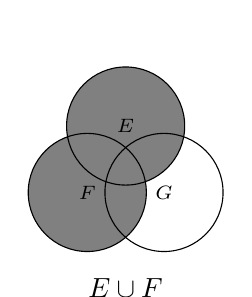
\begin{tikzpicture}[scale=0.75]
    \fill[fill=black!50] ( 90:.75) circle (1) (210:.75) circle (1);
    \foreach \a/\l in {90/E,210/F,330/G} {
        \path[draw] ++(\a:.75) circle (1) node {$\scriptstyle \l$};
    }
    \node at (0, -2) {$E \cup F$};
    \end{tikzpicture}
    \hspace{1em}
    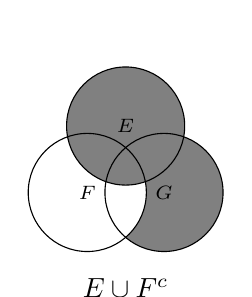
\begin{tikzpicture}[scale=0.75]
    \fill[fill=black!50] (90:.75) circle (1);
    \scope[even odd rule]
        \clip ( 90:.75) circle (1) (330:.75) circle (1);
        \clip (210:.75) circle (1) (330:.75) circle (1);
        \fill[fill=black!50] (330:.75) circle (1);
    \endscope
    \foreach \a/\l in {90/E,210/F,330/G} {
        \path[draw] ++(\a:.75) circle (1) node {$\scriptstyle \l$};
    }
    \node at (0, -2) {$E \cup F^c$};
    \end{tikzpicture}
    \]
    su intersección
    \[
    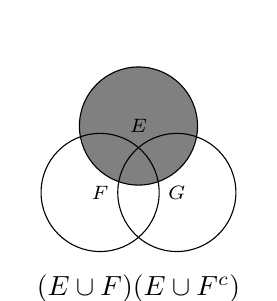
\begin{tikzpicture}[scale=0.75]
    \fill[fill=black!50] (90:.75) circle (1);
    \foreach \a/\l in {90/E,210/F,330/G} {
        \path[draw] ++(\a:.75) circle (1) node {$\scriptstyle \l$};
    }
    \node at (0, -2) {$(E \cup F) (E \cup F^c)$};
    \end{tikzpicture}
    \]
    \item to prove DeMorgan’s laws for events $E$ and $F$. (prove $(E \cup F)^c = E^cF^c$, and $(EF)^c = E^c \cup F^c$)

    \begin{proof}[Demostración] $(E \cup F)^c = E^cF^c$
        \[
        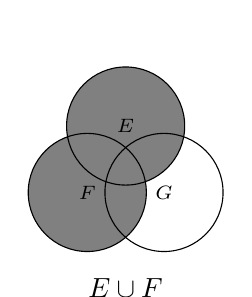
\begin{tikzpicture}[scale=0.75]
        \fill[fill=black!50] ( 90:.75) circle (1) (210:.75) circle (1);
        \foreach \a/\l in {90/E,210/F,330/G} {
            \path[draw] ++(\a:.75) circle (1) node {$\scriptstyle \l$};
        }
        \node at (0, -2) {$E \cup F$};
        \end{tikzpicture}
        \]
        su complemento
        \[
        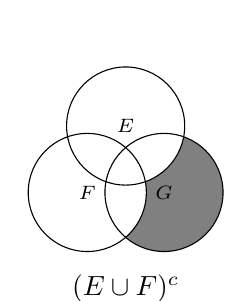
\begin{tikzpicture}[scale=0.75]
        \scope[even odd rule]
            \clip ( 90:.75) circle (1) (330:.75) circle (1);
            \clip (210:.75) circle (1) (330:.75) circle (1);
            \fill[fill=black!50] (330:.75) circle (1);
        \endscope
        \foreach \a/\l in {90/E,210/F,330/G} {
            \path[draw] ++(\a:.75) circle (1) node {$\scriptstyle \l$};
        }
        \node at (0, -2) {$(E \cup F)^c$};
        \end{tikzpicture}
        \]
        \[
        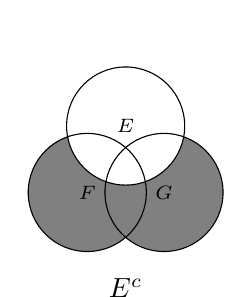
\begin{tikzpicture}[scale=0.75]
        \scope[even odd rule]
            \clip (210:.75) circle (1) (330:.75) circle (1);
            \clip ( 90:.75) circle (1) (210:.75) circle (1);
            \fill[fill=black!50] (210:.75) circle (1);
        \endscope
        \scope[even odd rule]
            \clip ( 90:.75) circle (1) (330:.75) circle (1);
            \fill[fill=black!50] (330:.75) circle (1);
        \endscope
        \foreach \a/\l in {90/E,210/F,330/G} {
            \path[draw] ++(\a:.75) circle (1) node {$\scriptstyle \l$};
        }
        \node at (0, -2) {$E^c$};
        \end{tikzpicture}
        \hspace{1em}
        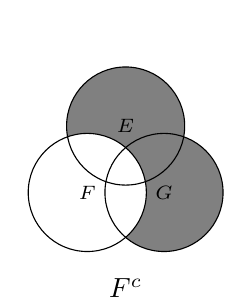
\begin{tikzpicture}[scale=0.75]
        \scope[even odd rule]
            \clip ( 90:.75) circle (1) (210:.75) circle (1);
            \clip (330:.75) circle (1) ( 90:.75) circle (1);
            \fill[fill=black!50] ( 90:.75) circle (1);
        \endscope
        \scope[even odd rule]
            \clip (210:.75) circle (1) (330:.75) circle (1);
            \fill[fill=black!50] (330:.75) circle (1);
        \endscope
        \foreach \a/\l in {90/E,210/F,330/G} {
            \path[draw] ++(\a:.75) circle (1) node {$\scriptstyle \l$};
        }
        \node at (0, -2) {$F^c$};
        \end{tikzpicture}
        \]
        su intersección
        \[
        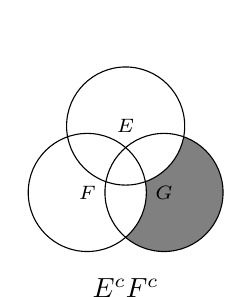
\begin{tikzpicture}[scale=0.75]
        \scope[even odd rule]
            \clip ( 90:.75) circle (1) (330:.75) circle (1);
            \clip (210:.75) circle (1) (330:.75) circle (1);
            \fill[fill=black!50] (330:.75) circle (1);
        \endscope
        \foreach \a/\l in {90/E,210/F,330/G} {
            \path[draw] ++(\a:.75) circle (1) node {$\scriptstyle \l$};
        }
        \node at (0, -2) {$E^c F^c$};
        \end{tikzpicture}
        \qedhere \]
    \end{proof}
    
    
    \begin{proof}[Demostración] $(EF)^c = E^c \cup F^c$
        \[
        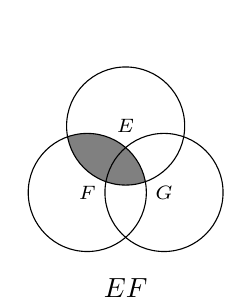
\begin{tikzpicture}[scale=0.75]
        \scope
            \clip (210:.75) circle (1);
            \fill[fill=black!50] ( 90:.75) circle (1);
        \endscope
        \foreach \a/\l in {90/E,210/F,330/G} {
            \path[draw] ++(\a:.75) circle (1) node {$\scriptstyle \l$};
        }
        \node at (0, -2) {$EF$};
        \end{tikzpicture}
        \]
        su complemento
        \[
        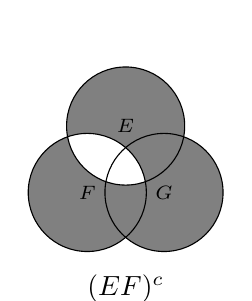
\begin{tikzpicture}[scale=0.75]
        \scope[even odd rule]
            \clip ( 90:.75) circle (1) (210:.75) circle (1);
            \fill[fill=black!50] (210:.75) circle (1);
        \endscope
        \scope[even odd rule]
            \clip ( 90:.75) circle (1) (210:.75) circle (1);
            \fill[fill=black!50] (90:.75) circle (1);
        \endscope
        \scope[even odd rule]
            \clip ( 90:.75) circle (1) (330:.75) circle (1);
            \clip (210:.75) circle (1) (330:.75) circle (1);
            \fill[fill=black!50] (330:.75) circle (1);
        \endscope
        \foreach \a/\l in {90/E,210/F,330/G} {
            \path[draw] ++(\a:.75) circle (1) node {$\scriptstyle \l$};
        }
        \node at (0, -2) {$(EF)^c$};
        \end{tikzpicture}
        \]
        \[
        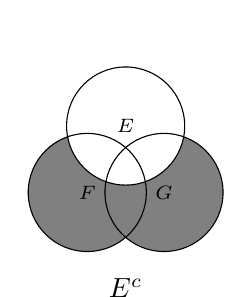
\begin{tikzpicture}[scale=0.75]
        \scope[even odd rule]
            \clip (210:.75) circle (1) (330:.75) circle (1);
            \clip ( 90:.75) circle (1) (210:.75) circle (1);
            \fill[fill=black!50] (210:.75) circle (1);
        \endscope
        \scope[even odd rule]
            \clip ( 90:.75) circle (1) (330:.75) circle (1);
            \fill[fill=black!50] (330:.75) circle (1);
        \endscope
        \foreach \a/\l in {90/E,210/F,330/G} {
            \path[draw] ++(\a:.75) circle (1) node {$\scriptstyle \l$};
        }
        \node at (0, -2) {$E^c$};
        \end{tikzpicture}
        \hspace{1em}
        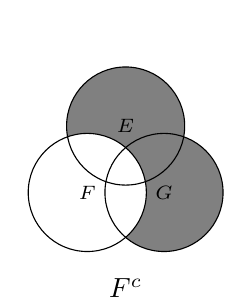
\begin{tikzpicture}[scale=0.75]
        \scope[even odd rule]
            \clip ( 90:.75) circle (1) (210:.75) circle (1);
            \clip (330:.75) circle (1) ( 90:.75) circle (1);
            \fill[fill=black!50] ( 90:.75) circle (1);
        \endscope
        \scope[even odd rule]
            \clip (210:.75) circle (1) (330:.75) circle (1);
            \fill[fill=black!50] (330:.75) circle (1);
        \endscope
        \foreach \a/\l in {90/E,210/F,330/G} {
            \path[draw] ++(\a:.75) circle (1) node {$\scriptstyle \l$};
        }
        \node at (0, -2) {$F^c$};
        \end{tikzpicture}
        \]
        su unión
        \[
        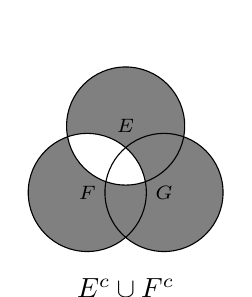
\begin{tikzpicture}[scale=0.75]
        \scope[even odd rule]
            \clip ( 90:.75) circle (1) (210:.75) circle (1);
            \fill[fill=black!50] (210:.75) circle (1);
        \endscope
        \scope[even odd rule]
            \clip ( 90:.75) circle (1) (210:.75) circle (1);
            \fill[fill=black!50] (90:.75) circle (1);
        \endscope
        \scope[even odd rule]
            \clip ( 90:.75) circle (1) (330:.75) circle (1);
            \clip (210:.75) circle (1) (330:.75) circle (1);
            \fill[fill=black!50] (330:.75) circle (1);
        \endscope
        \foreach \a/\l in {90/E,210/F,330/G} {
            \path[draw] ++(\a:.75) circle (1) node {$\scriptstyle \l$};
        }
        \node at (0, -2) {$E^c \cup F^c$};
        \end{tikzpicture} \qedhere
        \]
    \end{proof}
    
    
\end{enumerate}

    \item Suppose that $A$ and $B$ are mutually exclusive events for which $P(A) = .3$ and $P(B) = .5$. What is the probability that
\begin{enumerate}
    \item either $A$ or $B$ occurs?
    \begin{align*}
        P(A\cup B)
        &= P(A) + P(B)\\
        &= .3 + .5\\
        &= .8
    \end{align*}
    \item $A$ occurs but $B$ does not?
    \begin{align*}
        P(AB^\complement )
        &= P(A) - P(AB)\\
        &= .3 - .0\\
        &= .3
    \end{align*}
    \item both $A$ and $B$ occur?
    \begin{align*}
        P(AB) &= 0
    \end{align*}
\end{enumerate}
    \item A retail establishment accepts either the American Express or the VISA credit card. A total of 24 percent of its customers carry an American Express card, 61 percent carry a VISA card, and 11 percent carry both cards. What percentage of its customers carry a credit card that the establishment will accept?
\begin{align*}
    P(A\cup V) &= P(A) + P(V) - P(A \cap V)\\
    &= .24 + .61 - .11\\
    &= .74
\end{align*}
    \item In how many ways can 8 people be seated in a row if
\begin{enumerate}
    \item there are no restrictions on the seating arrangement?
    \[ 8! \]
    \item persons A and B must sit next to each other?
    \[ 2 * 7!\]
    \item there are 4 men and 4 women and no 2 men or 2 women can sit next to each other?

    Siguiendo la lógica de 7. iv.
    \[ 8 * 4 * 3 * 3 * 2 * 2 \]
    \item there are 5 men and they must sit next to one another?

    Hay $5!$ formas de sentar a los hombres entre sí, luego $4!$ formas de ordenar el grupo de hombres y las 3 mujeres.
    \[ 5! * 4! \]
    
    \item there are 4 married couples and each couple must sit together?

    Cada pareja tiene 2 formas de sentarse, luego hay $4!$ formas de ubicar a las parejas.
    \[ 2^4 * 4! \]
\end{enumerate}
    \item In how many ways can 3 novels, 2 mathematics books, and 1 chemistry book be arranged on a bookshelf if
\begin{enumerate}
    \item the books can be arranged in any order?
    \[ 6! \]
    \item the mathematics books must be together and the novels must be together?
    \[ 3! * 2! * 3! \]
    \item the novels must be together, but the other books can be arranged in any order?
    \[ 3! * 4! \]
\end{enumerate}
    \item A basketball team consists of 6 frontcourt and 4 backcourt players. If players are divided into roommates at random, what is the probability that there will be exactly two roommate pairs made up of a backcourt and a frontcourt player?
\[ \frac{\binom{6}{2} \binom{4}{2} * 2 * 3}{\frac{\binom{10}{2,2,2,2,2}}{5!}} \]
    \item Suppose that a person chooses a letter at random from R\,E\,S\,E\,R\,V\,E and then chooses one at random from \,V\,E\,R\,T\,I\,C\,A\,L. What is the probability that the same letter is chosen?
\[ 
\tfrac{2}{7} * \tfrac{1}{8} + \tfrac{3}{7} * \tfrac{1}{8} +
\tfrac{1}{7} * \tfrac{0}{8} + \tfrac{1}{7} * \tfrac{1}{8} = \tfrac{3}{28}  \]
    \item From a set of $n$ people, a committee of size $j$ is to be chosen, and from this committee, a subcommittee of size $i$, $i \le j$ is also to be chosen.
\begin{enumerate}
    \item Derive a combinatorial identity by computing, in two ways, the number of possible choices of the committee and subcommittee—first by supposing that the committee is chosen first and then the subcommittee is chosen, and second by supposing that the subcommittee is chosen first and then the remaining members of the committee are chosen.
    
    Supongamos que primero seleccionamos el comité, hay $\displaystyle \binom{n}{j}$ posibles comités, y de estas $j$ personas debemos seleccionar $i$ para que formen parte del subcomité
    \[ \binom{n}{j} * \binom{j}{i} \]

    Supongamos que primero seleccionamos el subcomité, hay $\displaystyle \binom{n}{i}$ posibles subcomités, luego de las restantes $n-i$ personas debemos seleccionar $j-i$
    \[ \binom{n}{i} * \binom{n-i}{j-i} \]

    Finalmente concluimos que
    \[ \binom{n}{j} * \binom{j}{i} = \binom{n}{i} * \binom{n-i}{j-i} \]

    \item Use part i. to prove the following combinatorial identity:
    \[ \sum_{j=i}^n \binom{n}{j} \binom{j}{i} = \binom{n}{i} * 2^{n-i} \quad i \le n \]
    \begin{align*}
        \shortintertext{por el inciso i.}
        \sum_{j=i}^n \binom{n}{j} \binom{j}{i} &= \sum_{j=i}^n \binom{n}{i} \binom{n-i}{j-i}\\
        &= \binom{n}{i} \sum_{j=i}^n \binom{n-i}{j-i}\\
        &= \binom{n}{i} \sum_{k=0}^{n-i} \binom{n-i}{k}
        \shortintertext{la suma equivale a todos los posibles subconjuntos de un conjunto con $n-i$ elementos.}
        &= \binom{n}{i} * 2^{n-i}
    \end{align*}
    
    \item  Use part i. and Theoretical Exercise 13 to show that
    \[ \sum_{j=i}^n \binom{n}{j} \binom{j}{i} (-1)^{(n-j)} = 0 \quad i < n\]
    \begin{align*}
        \shortintertext{por el inciso i.}
        &\phantom{{}={}} \sum_{j=i}^n \binom{n}{j} \binom{j}{i} (-1)^{(n-j)}\\
        &= \sum_{j=i}^n \binom{n}{i} \binom{n-i}{j-i} (-1)^{(n-j)}
        \shortintertext{la suma equivale a todos los posibles subconjuntos de un conjunto con $n-i$ elementos.}
        &= \binom{n}{i} * 2^{n-i}
    \end{align*}
\end{enumerate}
    \item A total of $n$ students are enrolled in a review course for the actuarial examination in probability. The posted results of the examination will list the names of those who passed, in decreasing order of their scores. For instance, the posted result will be \enquote{Brown, Cho} if Brown and Cho are the only ones to pass, with Brown receiving the higher score. Assuming that all scores are distinct (no ties), how many posted results are possible?
\[
\sum_{i=0}^n \binom{n}{i} * i!
\]
    \item Poker dice is played by simultaneously rolling 5 dice. Show that
\begin{enumerate}
    \item $P$\{no two alike\} = .0926;
    \[ \frac{6!}{6^5} \]
    \item $P$\{one pair\} = .4630;
    \[ \frac{\binom{6}{1} * 5 * 4 * 3 * \binom{5}{2}}{6^6} \]
    \item $P$\{two pair\} = .2315;
    \[ \frac{\binom{6}{2} * 4 * \frac{5!}{2!*2!}}{6^5} \]
    \item $P$\{three alike\} = .1543;
    \[ \frac{\binom{6}{1} * 5 * 4 * \binom{5}{3}}{6^5} \]
    \item $P$\{full house\} = .0386;
    \[ \frac{6 * 5 * \binom{5}{3}}{6^5} \]
    \item $P$\{four alike\} = .0193;
    \[ \frac{6 * 5 * 5}{6^5} \]
    \item $P$\{five alike\} = .0008.
    \[ \frac{6}{6^5} \]
\end{enumerate}
    \item Present a combinatorial explanation of why
\[ \binom{n}{r} = \binom{n}{r, n-r} \]

Al seleccionar $r$ objetos entre $n$ objetos queda únicamente determinado otro grupo de $n-r$ objetos, los que no fueron seleccionados.
    \item Two cards are randomly selected from an ordinary playing deck. What is the probability that they form a blackjack? That is, what is the probability that one of the cards is an ace and the other one is either a ten, a jack, a queen, or a king?
\[
\frac{4 * 4 * 4}{\binom{52}{2}}
\]
    \item If there are no restrictions on where the digits and letters are placed, how many 8-place license plates consisting of 5 letters and 3 digits are possible if no repetitions of letters or digits are allowed? What if the 3 digits must be consecutive?
\[ \binom{8}{3} * \frac{26!}{21!} * \frac{10!}{7!} \]
Si los 3 dígitos deben ser consecutivos entonces
\[ 6 * \frac{26!}{21!} * \frac{10!}{7!} \]
    \item In how many ways can $n$ identical balls be distributed into $r$ urns so that the $i$th urn contains at least $m_i$ balls for each $i = 1,\dots,r$? Assume that $n \ge \sum_{i=1}^r m_i$.

Primero colocamos las bolillas requeridas en las urnas, y nos restan $n - \sum_{i=1}^r m_i$ bolillas.

Luego debemos colocar las $n - \sum_{i=1}^r m_i$ bolillas restantes en las $r$ urnas
\[ \binom{ n + r - 1 - \sum_{i=1}^r m_i}{r-1} \]
    \item A small community organization consists of 20 families, of which 4 have one child, 8 have two children, 5 have three children, 2 have four children, and 1 has five children.

%4+2*8+3*5+4*2+5*1=20+23+5=48

\begin{enumerate}
    \item If one of these families is chosen at random, what is the probability it has $i$ children, $i = 1,2,3,4,5$?
    \[ 1.\ \frac{4}{20} \quad 2.\ \frac{8}{20} \quad 3.\ \frac{5}{20} \quad 4.\ \frac{2}{20} \quad 5.\ \frac{1}{20} \quad \]
    \item If one of the children is randomly chosen, what is the probability that child comes from a family having $i$ children, $i = 1,2,3,4,5$?
    \[ 1.\ \frac{4}{48} \quad 2.\ \frac{16}{48} \quad 3.\ \frac{15}{48} \quad 4.\ \frac{8}{48} \quad 5.\ \frac{5}{48} \quad \]
\end{enumerate}
\end{enumerate}
    
\section*{Self-Test Problems}
\begin{enumerate}
    \item  A cafeteria offers a three-course meal consisting of an entree, a starch, and a dessert. The possible choices aregiven in the following table

\[
{
\begin{tabular}{ll}
    \hline
    \multicolumn{1}{c}{Course} & \multicolumn{1}{c}{Choices} \\
    \hline
    Entree & Chicken Roast, Roast Beef\\
    Starch & Pasta, rice, potatoes\\
    Dessert & Ice cream, Jello, apple pie, a peach\\
    \hline
\end{tabular}
}
\]
A person is to choose one course from each category.
\begin{enumerate}
    \item How many outcomes are in the sample space?
    \[ 2 * 3 * 4 \]
    \item Let $A$ be the event that ice cream is chosen. How many outcomes are in $A$?
    \[ 2 * 3 \]
    \item Let $B$ be the event that chicken is chosen. How many outcomes are in $B$?
    \[ 3 * 4 \]
    \item List all the outcomes in the event $AB$.
    \begin{align*}
        AB = \{ &\text{(chicken, pasta, ice-cream)},\\
        &\text{(chicken, rice, ice-cream)},\\
        &\text{(chicken, potatoes, ice-cream)} \}
    \end{align*}
    \item Let $C$ be the event that rice is chosen. How many outcomes are in $C$?
    \[ 2 * 4 \]
    \item List all the outcomes in the event $ABC$.
    \[ ABC = \{ \text{(chicken, rice, ice-cream)} \} \]
\end{enumerate}

    \item If 4 Americans, 3 French people, and 3 British people are to be seated in a row, how many seating arrangements are possible when people of the same nationality must sit next to each other?
\[ 4! * 3! * 3! * 3! \]
    \item $F = FE \cup FE^\complement $ and $E \cup F = E \cup E^\complement F$.

\begin{proof}[Demostración] de la relación anterior.

    \begin{align*}
        F &= FS\\
        &= F (E\cup E^\complement )\\
        &= FE \cup F E^\complement 
        \shortintertext{y}
        E \cup F &= (E \cup F)(E\cup E^\complement )\\
        &= ((E\cup F)E) \cup ((E\cup F)E^\complement )\\
        &= E \cup ((E^\complement  E)\cup(E^\complement  F))\\
        &= E \cup (\varnothing\cup(E^\complement  F))\\
        &= E \cup E^\complement  F \qedhere
    \end{align*}
\end{proof}
    \item $A$, $B$, and $C$ take turns flipping a coin. The first one to get a head wins. The sample space of this experiment can be defined by
\[ S = \begin{cases}
    1, 01, 001, 0001, \dots,\\
    0000\cdots
\end{cases} \]
\begin{enumerate}
    \item Interpret the sample space.
    
    Es el conjunto de secuencias formadas por 0 y 1, donde el $i$-ésimo componente representa el resultado de la tirada $i$-ésima, con 0 representando que el resultado es ceca y 1 representando que el resultado es cara. 
    
    \item Define the following events in terms of $S$, assuming that $A$ flips first, then $B$, then $C$, $\dots$
    \begin{enumerate}[label={\alph*.}]
        \item $A \text{ wins} = A.$
        \[ A = \set{ 1, 0001, 0000001, \dots } \]
        \item $B \text{ wins} = B.$
        \[ B = \set{ 01, 00001, 00000001, \dots } \]
        \item $(A \cup B)^\complement $
        \[ (A \cup B)^\complement  = \begin{cases}
            &001, 000001, \dots\\
            &0000\cdots
        \end{cases} \]
    \end{enumerate}
\end{enumerate}
    \item An ordinary deck of 52 cards is shuffled. What is the probability that the top four cards have
\begin{enumerate}
    \item different denominations?
    \[ \frac{\binom{13}{4}\binom{4}{1}^4}{\binom{52}{4}} \]
    \item different suits?
    \[ \frac{\binom{13}{1}^4}{\binom{52}{4}} \]
\end{enumerate}

    \item How many vectors $x_1, \dots, x_k$ are there for which each $x_i$ is a positive integer such that $1 \le x_i \le n$ and $x_1 < x_2 < \dots < x_k$?

Seleccionar los $k+i$ primeros números, y entre ellos asignar a $i$ el estatus de \enquote{ignorado}.
\[ \sum_{i=0}^{n-k} \binom{k+i}{i} \]
    \item Use Venn diagrams
\begin{enumerate}
    \item to simplify $(E \cup F)(E \cup F^c)$
    \[
    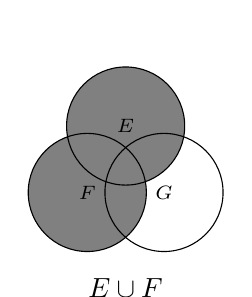
\begin{tikzpicture}[scale=0.75]
    \fill[fill=black!50] ( 90:.75) circle (1) (210:.75) circle (1);
    \foreach \a/\l in {90/E,210/F,330/G} {
        \path[draw] ++(\a:.75) circle (1) node {$\scriptstyle \l$};
    }
    \node at (0, -2) {$E \cup F$};
    \end{tikzpicture}
    \hspace{1em}
    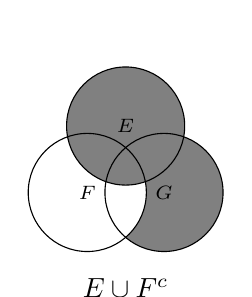
\begin{tikzpicture}[scale=0.75]
    \fill[fill=black!50] (90:.75) circle (1);
    \scope[even odd rule]
        \clip ( 90:.75) circle (1) (330:.75) circle (1);
        \clip (210:.75) circle (1) (330:.75) circle (1);
        \fill[fill=black!50] (330:.75) circle (1);
    \endscope
    \foreach \a/\l in {90/E,210/F,330/G} {
        \path[draw] ++(\a:.75) circle (1) node {$\scriptstyle \l$};
    }
    \node at (0, -2) {$E \cup F^c$};
    \end{tikzpicture}
    \]
    su intersección
    \[
    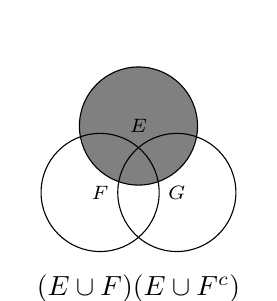
\begin{tikzpicture}[scale=0.75]
    \fill[fill=black!50] (90:.75) circle (1);
    \foreach \a/\l in {90/E,210/F,330/G} {
        \path[draw] ++(\a:.75) circle (1) node {$\scriptstyle \l$};
    }
    \node at (0, -2) {$(E \cup F) (E \cup F^c)$};
    \end{tikzpicture}
    \]
    \item to prove DeMorgan’s laws for events $E$ and $F$. (prove $(E \cup F)^c = E^cF^c$, and $(EF)^c = E^c \cup F^c$)

    \begin{proof}[Demostración] $(E \cup F)^c = E^cF^c$
        \[
        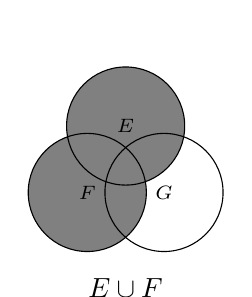
\begin{tikzpicture}[scale=0.75]
        \fill[fill=black!50] ( 90:.75) circle (1) (210:.75) circle (1);
        \foreach \a/\l in {90/E,210/F,330/G} {
            \path[draw] ++(\a:.75) circle (1) node {$\scriptstyle \l$};
        }
        \node at (0, -2) {$E \cup F$};
        \end{tikzpicture}
        \]
        su complemento
        \[
        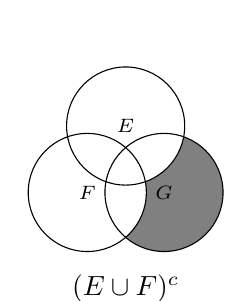
\begin{tikzpicture}[scale=0.75]
        \scope[even odd rule]
            \clip ( 90:.75) circle (1) (330:.75) circle (1);
            \clip (210:.75) circle (1) (330:.75) circle (1);
            \fill[fill=black!50] (330:.75) circle (1);
        \endscope
        \foreach \a/\l in {90/E,210/F,330/G} {
            \path[draw] ++(\a:.75) circle (1) node {$\scriptstyle \l$};
        }
        \node at (0, -2) {$(E \cup F)^c$};
        \end{tikzpicture}
        \]
        \[
        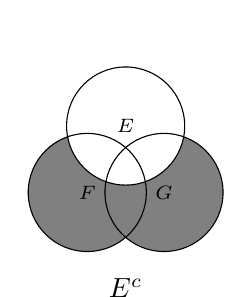
\begin{tikzpicture}[scale=0.75]
        \scope[even odd rule]
            \clip (210:.75) circle (1) (330:.75) circle (1);
            \clip ( 90:.75) circle (1) (210:.75) circle (1);
            \fill[fill=black!50] (210:.75) circle (1);
        \endscope
        \scope[even odd rule]
            \clip ( 90:.75) circle (1) (330:.75) circle (1);
            \fill[fill=black!50] (330:.75) circle (1);
        \endscope
        \foreach \a/\l in {90/E,210/F,330/G} {
            \path[draw] ++(\a:.75) circle (1) node {$\scriptstyle \l$};
        }
        \node at (0, -2) {$E^c$};
        \end{tikzpicture}
        \hspace{1em}
        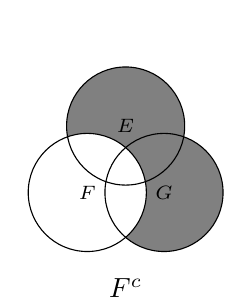
\begin{tikzpicture}[scale=0.75]
        \scope[even odd rule]
            \clip ( 90:.75) circle (1) (210:.75) circle (1);
            \clip (330:.75) circle (1) ( 90:.75) circle (1);
            \fill[fill=black!50] ( 90:.75) circle (1);
        \endscope
        \scope[even odd rule]
            \clip (210:.75) circle (1) (330:.75) circle (1);
            \fill[fill=black!50] (330:.75) circle (1);
        \endscope
        \foreach \a/\l in {90/E,210/F,330/G} {
            \path[draw] ++(\a:.75) circle (1) node {$\scriptstyle \l$};
        }
        \node at (0, -2) {$F^c$};
        \end{tikzpicture}
        \]
        su intersección
        \[
        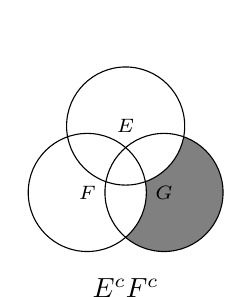
\begin{tikzpicture}[scale=0.75]
        \scope[even odd rule]
            \clip ( 90:.75) circle (1) (330:.75) circle (1);
            \clip (210:.75) circle (1) (330:.75) circle (1);
            \fill[fill=black!50] (330:.75) circle (1);
        \endscope
        \foreach \a/\l in {90/E,210/F,330/G} {
            \path[draw] ++(\a:.75) circle (1) node {$\scriptstyle \l$};
        }
        \node at (0, -2) {$E^c F^c$};
        \end{tikzpicture}
        \qedhere \]
    \end{proof}
    
    
    \begin{proof}[Demostración] $(EF)^c = E^c \cup F^c$
        \[
        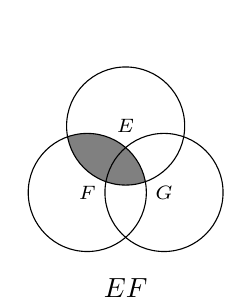
\begin{tikzpicture}[scale=0.75]
        \scope
            \clip (210:.75) circle (1);
            \fill[fill=black!50] ( 90:.75) circle (1);
        \endscope
        \foreach \a/\l in {90/E,210/F,330/G} {
            \path[draw] ++(\a:.75) circle (1) node {$\scriptstyle \l$};
        }
        \node at (0, -2) {$EF$};
        \end{tikzpicture}
        \]
        su complemento
        \[
        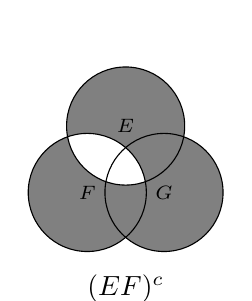
\begin{tikzpicture}[scale=0.75]
        \scope[even odd rule]
            \clip ( 90:.75) circle (1) (210:.75) circle (1);
            \fill[fill=black!50] (210:.75) circle (1);
        \endscope
        \scope[even odd rule]
            \clip ( 90:.75) circle (1) (210:.75) circle (1);
            \fill[fill=black!50] (90:.75) circle (1);
        \endscope
        \scope[even odd rule]
            \clip ( 90:.75) circle (1) (330:.75) circle (1);
            \clip (210:.75) circle (1) (330:.75) circle (1);
            \fill[fill=black!50] (330:.75) circle (1);
        \endscope
        \foreach \a/\l in {90/E,210/F,330/G} {
            \path[draw] ++(\a:.75) circle (1) node {$\scriptstyle \l$};
        }
        \node at (0, -2) {$(EF)^c$};
        \end{tikzpicture}
        \]
        \[
        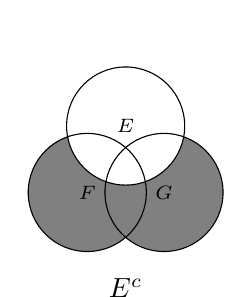
\begin{tikzpicture}[scale=0.75]
        \scope[even odd rule]
            \clip (210:.75) circle (1) (330:.75) circle (1);
            \clip ( 90:.75) circle (1) (210:.75) circle (1);
            \fill[fill=black!50] (210:.75) circle (1);
        \endscope
        \scope[even odd rule]
            \clip ( 90:.75) circle (1) (330:.75) circle (1);
            \fill[fill=black!50] (330:.75) circle (1);
        \endscope
        \foreach \a/\l in {90/E,210/F,330/G} {
            \path[draw] ++(\a:.75) circle (1) node {$\scriptstyle \l$};
        }
        \node at (0, -2) {$E^c$};
        \end{tikzpicture}
        \hspace{1em}
        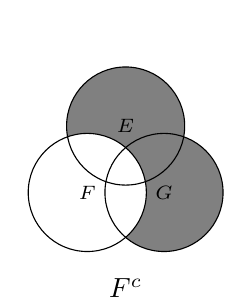
\begin{tikzpicture}[scale=0.75]
        \scope[even odd rule]
            \clip ( 90:.75) circle (1) (210:.75) circle (1);
            \clip (330:.75) circle (1) ( 90:.75) circle (1);
            \fill[fill=black!50] ( 90:.75) circle (1);
        \endscope
        \scope[even odd rule]
            \clip (210:.75) circle (1) (330:.75) circle (1);
            \fill[fill=black!50] (330:.75) circle (1);
        \endscope
        \foreach \a/\l in {90/E,210/F,330/G} {
            \path[draw] ++(\a:.75) circle (1) node {$\scriptstyle \l$};
        }
        \node at (0, -2) {$F^c$};
        \end{tikzpicture}
        \]
        su unión
        \[
        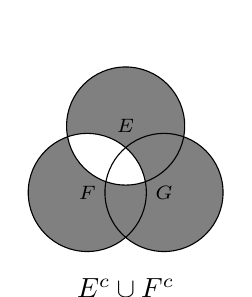
\begin{tikzpicture}[scale=0.75]
        \scope[even odd rule]
            \clip ( 90:.75) circle (1) (210:.75) circle (1);
            \fill[fill=black!50] (210:.75) circle (1);
        \endscope
        \scope[even odd rule]
            \clip ( 90:.75) circle (1) (210:.75) circle (1);
            \fill[fill=black!50] (90:.75) circle (1);
        \endscope
        \scope[even odd rule]
            \clip ( 90:.75) circle (1) (330:.75) circle (1);
            \clip (210:.75) circle (1) (330:.75) circle (1);
            \fill[fill=black!50] (330:.75) circle (1);
        \endscope
        \foreach \a/\l in {90/E,210/F,330/G} {
            \path[draw] ++(\a:.75) circle (1) node {$\scriptstyle \l$};
        }
        \node at (0, -2) {$E^c \cup F^c$};
        \end{tikzpicture} \qedhere
        \]
    \end{proof}
    
    
\end{enumerate}

    \item Suppose that $A$ and $B$ are mutually exclusive events for which $P(A) = .3$ and $P(B) = .5$. What is the probability that
\begin{enumerate}
    \item either $A$ or $B$ occurs?
    \begin{align*}
        P(A\cup B)
        &= P(A) + P(B)\\
        &= .3 + .5\\
        &= .8
    \end{align*}
    \item $A$ occurs but $B$ does not?
    \begin{align*}
        P(AB^\complement )
        &= P(A) - P(AB)\\
        &= .3 - .0\\
        &= .3
    \end{align*}
    \item both $A$ and $B$ occur?
    \begin{align*}
        P(AB) &= 0
    \end{align*}
\end{enumerate}
    \item A retail establishment accepts either the American Express or the VISA credit card. A total of 24 percent of its customers carry an American Express card, 61 percent carry a VISA card, and 11 percent carry both cards. What percentage of its customers carry a credit card that the establishment will accept?
\begin{align*}
    P(A\cup V) &= P(A) + P(V) - P(A \cap V)\\
    &= .24 + .61 - .11\\
    &= .74
\end{align*}
    \item In how many ways can 8 people be seated in a row if
\begin{enumerate}
    \item there are no restrictions on the seating arrangement?
    \[ 8! \]
    \item persons A and B must sit next to each other?
    \[ 2 * 7!\]
    \item there are 4 men and 4 women and no 2 men or 2 women can sit next to each other?

    Siguiendo la lógica de 7. iv.
    \[ 8 * 4 * 3 * 3 * 2 * 2 \]
    \item there are 5 men and they must sit next to one another?

    Hay $5!$ formas de sentar a los hombres entre sí, luego $4!$ formas de ordenar el grupo de hombres y las 3 mujeres.
    \[ 5! * 4! \]
    
    \item there are 4 married couples and each couple must sit together?

    Cada pareja tiene 2 formas de sentarse, luego hay $4!$ formas de ubicar a las parejas.
    \[ 2^4 * 4! \]
\end{enumerate}
    \item In how many ways can 3 novels, 2 mathematics books, and 1 chemistry book be arranged on a bookshelf if
\begin{enumerate}
    \item the books can be arranged in any order?
    \[ 6! \]
    \item the mathematics books must be together and the novels must be together?
    \[ 3! * 2! * 3! \]
    \item the novels must be together, but the other books can be arranged in any order?
    \[ 3! * 4! \]
\end{enumerate}
    \item A basketball team consists of 6 frontcourt and 4 backcourt players. If players are divided into roommates at random, what is the probability that there will be exactly two roommate pairs made up of a backcourt and a frontcourt player?
\[ \frac{\binom{6}{2} \binom{4}{2} * 2 * 3}{\frac{\binom{10}{2,2,2,2,2}}{5!}} \]
    \item Suppose that a person chooses a letter at random from R\,E\,S\,E\,R\,V\,E and then chooses one at random from \,V\,E\,R\,T\,I\,C\,A\,L. What is the probability that the same letter is chosen?
\[ 
\tfrac{2}{7} * \tfrac{1}{8} + \tfrac{3}{7} * \tfrac{1}{8} +
\tfrac{1}{7} * \tfrac{0}{8} + \tfrac{1}{7} * \tfrac{1}{8} = \tfrac{3}{28}  \]
    \item From a set of $n$ people, a committee of size $j$ is to be chosen, and from this committee, a subcommittee of size $i$, $i \le j$ is also to be chosen.
\begin{enumerate}
    \item Derive a combinatorial identity by computing, in two ways, the number of possible choices of the committee and subcommittee—first by supposing that the committee is chosen first and then the subcommittee is chosen, and second by supposing that the subcommittee is chosen first and then the remaining members of the committee are chosen.
    
    Supongamos que primero seleccionamos el comité, hay $\displaystyle \binom{n}{j}$ posibles comités, y de estas $j$ personas debemos seleccionar $i$ para que formen parte del subcomité
    \[ \binom{n}{j} * \binom{j}{i} \]

    Supongamos que primero seleccionamos el subcomité, hay $\displaystyle \binom{n}{i}$ posibles subcomités, luego de las restantes $n-i$ personas debemos seleccionar $j-i$
    \[ \binom{n}{i} * \binom{n-i}{j-i} \]

    Finalmente concluimos que
    \[ \binom{n}{j} * \binom{j}{i} = \binom{n}{i} * \binom{n-i}{j-i} \]

    \item Use part i. to prove the following combinatorial identity:
    \[ \sum_{j=i}^n \binom{n}{j} \binom{j}{i} = \binom{n}{i} * 2^{n-i} \quad i \le n \]
    \begin{align*}
        \shortintertext{por el inciso i.}
        \sum_{j=i}^n \binom{n}{j} \binom{j}{i} &= \sum_{j=i}^n \binom{n}{i} \binom{n-i}{j-i}\\
        &= \binom{n}{i} \sum_{j=i}^n \binom{n-i}{j-i}\\
        &= \binom{n}{i} \sum_{k=0}^{n-i} \binom{n-i}{k}
        \shortintertext{la suma equivale a todos los posibles subconjuntos de un conjunto con $n-i$ elementos.}
        &= \binom{n}{i} * 2^{n-i}
    \end{align*}
    
    \item  Use part i. and Theoretical Exercise 13 to show that
    \[ \sum_{j=i}^n \binom{n}{j} \binom{j}{i} (-1)^{(n-j)} = 0 \quad i < n\]
    \begin{align*}
        \shortintertext{por el inciso i.}
        &\phantom{{}={}} \sum_{j=i}^n \binom{n}{j} \binom{j}{i} (-1)^{(n-j)}\\
        &= \sum_{j=i}^n \binom{n}{i} \binom{n-i}{j-i} (-1)^{(n-j)}
        \shortintertext{la suma equivale a todos los posibles subconjuntos de un conjunto con $n-i$ elementos.}
        &= \binom{n}{i} * 2^{n-i}
    \end{align*}
\end{enumerate}
    \item A total of $n$ students are enrolled in a review course for the actuarial examination in probability. The posted results of the examination will list the names of those who passed, in decreasing order of their scores. For instance, the posted result will be \enquote{Brown, Cho} if Brown and Cho are the only ones to pass, with Brown receiving the higher score. Assuming that all scores are distinct (no ties), how many posted results are possible?
\[
\sum_{i=0}^n \binom{n}{i} * i!
\]
    \item Poker dice is played by simultaneously rolling 5 dice. Show that
\begin{enumerate}
    \item $P$\{no two alike\} = .0926;
    \[ \frac{6!}{6^5} \]
    \item $P$\{one pair\} = .4630;
    \[ \frac{\binom{6}{1} * 5 * 4 * 3 * \binom{5}{2}}{6^6} \]
    \item $P$\{two pair\} = .2315;
    \[ \frac{\binom{6}{2} * 4 * \frac{5!}{2!*2!}}{6^5} \]
    \item $P$\{three alike\} = .1543;
    \[ \frac{\binom{6}{1} * 5 * 4 * \binom{5}{3}}{6^5} \]
    \item $P$\{full house\} = .0386;
    \[ \frac{6 * 5 * \binom{5}{3}}{6^5} \]
    \item $P$\{four alike\} = .0193;
    \[ \frac{6 * 5 * 5}{6^5} \]
    \item $P$\{five alike\} = .0008.
    \[ \frac{6}{6^5} \]
\end{enumerate}
    \item Present a combinatorial explanation of why
\[ \binom{n}{r} = \binom{n}{r, n-r} \]

Al seleccionar $r$ objetos entre $n$ objetos queda únicamente determinado otro grupo de $n-r$ objetos, los que no fueron seleccionados.
    \item Two cards are randomly selected from an ordinary playing deck. What is the probability that they form a blackjack? That is, what is the probability that one of the cards is an ace and the other one is either a ten, a jack, a queen, or a king?
\[
\frac{4 * 4 * 4}{\binom{52}{2}}
\]
    \item If there are no restrictions on where the digits and letters are placed, how many 8-place license plates consisting of 5 letters and 3 digits are possible if no repetitions of letters or digits are allowed? What if the 3 digits must be consecutive?
\[ \binom{8}{3} * \frac{26!}{21!} * \frac{10!}{7!} \]
Si los 3 dígitos deben ser consecutivos entonces
\[ 6 * \frac{26!}{21!} * \frac{10!}{7!} \]
    \item In how many ways can $n$ identical balls be distributed into $r$ urns so that the $i$th urn contains at least $m_i$ balls for each $i = 1,\dots,r$? Assume that $n \ge \sum_{i=1}^r m_i$.

Primero colocamos las bolillas requeridas en las urnas, y nos restan $n - \sum_{i=1}^r m_i$ bolillas.

Luego debemos colocar las $n - \sum_{i=1}^r m_i$ bolillas restantes en las $r$ urnas
\[ \binom{ n + r - 1 - \sum_{i=1}^r m_i}{r-1} \]
\end{enumerate}

\end{document}
